\documentclass{standalone}
\usepackage{tikz}
\usepackage{ctex,siunitx}
\usepackage{tkz-euclide}
\usepackage{amsmath}
\usetikzlibrary{patterns, calc}
\usetikzlibrary {decorations.pathmorphing, decorations.pathreplacing, decorations.shapes,}
\begin{document}
\small
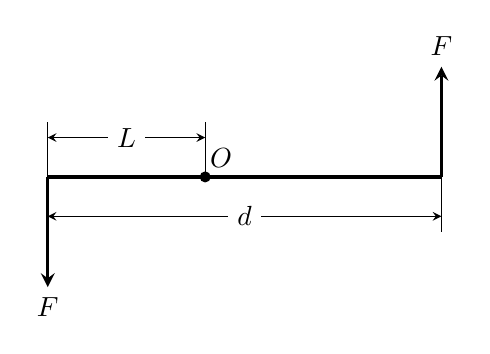
\begin{tikzpicture}[>=stealth,scale=1.0]
  \draw[ultra thick](-2,0)--(3,0);
  \node at (.2,0) [above]{$O$};
  \draw[->,very thick](-2,0)--(-2,-1.4) node [below]{$F$};
  \draw[->,very thick](3,0)--(3,1.4)node [above]{$F$};
  \draw[<->](-2,.5)--node [fill=white]{$L$} (0,.5);
  \draw[<->](-2,-.5)--node [fill=white]{$d$} (3,-.5);
  \fill (0,0) circle(2pt);
  \draw[thin](-2,0)--(-2,0.7);  
  \draw[thin](0,0)--(0,0.7); 
  \draw[thin](3,0)--(3,-0.7);
\end{tikzpicture}
\end{document}